\documentclass[14pt]{article}
\usepackage[margin=1.5cm]{geometry}
% Data flow diagram
% A custom data flow diagram environment
\usepackage{tikz}
\usetikzlibrary{arrows}

% Defines a max size for process bubbles
\newlength{\procsze}
\newcommand{\sizeprocess}[1]{
  \setlength{\procsze}{#1}
}

% Define a wrapper for tikz that has custom styles for data flow diagrams
\newenvironment{dfd}
{
\begin{tikzpicture}[
  x=2cm, y=2cm,
  font=\sffamily,
  every matrix/.style={ampersand replacement=\&,column sep=2cm,row sep=2cm},
  xtern/.style={draw,thick,inner sep=.3cm},
  process/.style={draw,thick,circle},
  sized/.style={minimum size=\procsze},
  datastore/.style={draw,very thick,shape=datastore,inner sep=.3cm},
  dots/.style={gray,scale=2},
  to/.style={->,>=stealth',shorten >=1pt,semithick,font=\sffamily\footnotesize},
  every node/.style={align=center}
]
}
{
\end{tikzpicture}
}

% Defines a `datastore' shape for use in DFDs.  This inherits from a
% rectangle and only draws two horizontal lines.
\makeatletter
\pgfdeclareshape{datastore}{
  \inheritsavedanchors[from=rectangle]
  \inheritanchorborder[from=rectangle]
  \inheritanchor[from=rectangle]{center}
  \inheritanchor[from=rectangle]{base}
  \inheritanchor[from=rectangle]{north}
  \inheritanchor[from=rectangle]{north east}
  \inheritanchor[from=rectangle]{east}
  \inheritanchor[from=rectangle]{south east}
  \inheritanchor[from=rectangle]{south}
  \inheritanchor[from=rectangle]{south west}
  \inheritanchor[from=rectangle]{west}
  \inheritanchor[from=rectangle]{north west}
  \backgroundpath{
    % store lower-left in xa/ya and upper-right in xb/yb
    \southwest \pgf@xa=\pgf@x \pgf@ya=\pgf@y
    \northeast \pgf@xb=\pgf@x \pgf@yb=\pgf@y

    % bottom line
    \pgfpathmoveto{\pgfpoint{\pgf@xa}{\pgf@ya}}
    \pgfpathlineto{\pgfpoint{\pgf@xb}{\pgf@ya}}

    % top line
    \pgfpathmoveto{\pgfpoint{\pgf@xa}{\pgf@yb}}
    \pgfpathlineto{\pgfpoint{\pgf@xb}{\pgf@yb}}

    % left vertical line
    \pgfpathmoveto{\pgfpoint{\pgf@xa}{\pgf@ya}}
    \pgfpathlineto{\pgfpoint{\pgf@xa}{\pgf@yb}}
  }
}
\makeatother

% Structure chart
% A custom structure chart environment
\usepackage{xparse}
\usepackage{tikz}
\usetikzlibrary{arrows}

% Define a wrapper for tikz that has custom styles for structure charts
\newenvironment{structc}
{
\begin{tikzpicture}[
  font=\sffamily,
  every matrix/.style={ampersand replacement=\&,column sep=2cm,row sep=2cm},
  module/.style={draw,thick,inner sep=.3cm},
  diamondmark/.style={draw,diamond,fill=white!10,minimum size=5mm,sloped,transform shape,xshift=2.5mm},
  repeat/.style={sloped,transform shape,anchor=center},
  data/.style={sloped,transform shape,yshift=2.5mm},
  to/.style={-,>=stealth',shorten >=1pt,semithick,font=\sffamily\footnotesize},
  every node/.style={align=center}
]
}
{
\end{tikzpicture}
}

\NewDocumentCommand{\dfdData}{O{white} m m O{0} O{south}}{
  \begin{tikzpicture}[baseline]
    \node[circle,draw,fill=#1,minimum size=3mm] (c) {};

    \pgfmathparse{#3>=0 ? "east" : "west"}
    \edef\anchor{\pgfmathresult}
    \draw[->,>=stealth',line width=0.5pt] (c.\anchor) -- ++(#3*2mm,0);

    \node[above=0.2mm of c,anchor=#5,rotate=#4,overlay] {\footnotesize #2};
  \end{tikzpicture}
}

\newcommand{\dfdLoop}[2][0.3]{
  \begin{tikzpicture}[baseline]
    \pgfmathsetmacro{\xscale}{-(1/#1)*0.5}
    \draw[->,>=stealth',thick,xscale=\xscale] (0,0) arc (30:330:#1);
    \node[anchor=east,align=center,rotate=90,overlay,yshift=-1mm] at (#1*-2*\xscale,\xscale) {\footnotesize #2};
  \end{tikzpicture}
}


% Be able to set bullet point styles
\usepackage{enumitem}

% Better tables
\usepackage{xltabular}
\NewDocumentEnvironment{brtbl}{ m m m }{%
  \xltabular{\textwidth}{#1}
    \hline
    #3 \\
    \hline\hline
    \endhead
    \multicolumn{#2}{c}{\emph{Continued on next page}}
    \endfoot
    \hline
    \endlastfoot
}{%
  \endxltabular
}

% Font
\usepackage[T1]{fontenc}
\usepackage[sfdefault]{atkinson}

% Custom commands
\newcommand{\todo}[1][finish]{%
  {\Large\hl{\textbf{TODO: #1}}}%
}
% Usage: \todo or \todo[This]

% Box around page
\usepackage{pgf}
\usepackage{pgfpages}
\pgfpagesdeclarelayout{boxed}
{
  \edef\pgfpageoptionborder{0pt}
}
{
  \pgfpagesphysicalpageoptions
  {%
    logical pages=1,%
  }
  \pgfpageslogicalpageoptions{1}
  {
    border code=\pgfsetlinewidth{2pt}\pgfstroke,%
    border shrink=\pgfpageoptionborder,%
    resized width=.95\pgfphysicalwidth,%
    resized height=.95\pgfphysicalheight,%
    center=\pgfpoint{.5\pgfphysicalwidth}{.5\pgfphysicalheight}%
  }%
}

\pgfpagesuselayout{boxed}

\usepackage{soul}

% Chart packages
\usepackage{float}
\usepackage{pgfgantt}

\author{Max Worrall}
\title{Quiet Space}

\begin{document}


\maketitle
\tableofcontents
\pagebreak


\section{Identifying and Defining}

\subsection{Problem Statement}
% Outline the problem or opportunity that the project addresses. Consider who is affected by this issue.
% Explain why this problem or opportunity is significant.
% Justify the development of a software solution as an appropriate response.
People have increasingly busy lifestyles, and during periods of downtime such as when waiting for public transport, when people are bored, or in many other scenarios - digital platforms have been optimised for user engagement and can increase stress and anxiety. For example, many apps (especially ones paying to show above search results and on the home screen of app stores to be more frequently downloaded) utilise lootboxes, repetitive gameplay loops and constantly make users come back with streaks and limited time events. These features are often created to increase user engagement to provide opportunity for microtransactions and company profit, even though it detriments users. Additionally, the internet is a source for a lot of potentially stressful news and FOMO-inducing social media, among many other things.

This is significant as these increases of stress in an already busy life can lead to negative consequences such as burnout, anxiety and other mental health issues. Developing a space designed to be consistently interesting (through curiosity) yet still relaxing can help solve this problem. Instead of spending free moments playing high-intensity mobile games or scrolling social media, people can instead play this game which decreases stress while remaining rewarding enough to encourage continued engagement. This is practical because it can be used in the same moments of downtime that would be filled with more stressful activities. Ultimately, this may contribute to an increased wellbeing in users by replacing more stressful digital games.

\subsection{Project Purpose and Boundaries}
% Outline what the project is trying to achieve.
The project will provide a relaxing digital space on the internet users can explore and build within. The game will consist of a procedurally generated world that varies in each new world, while utilising relaxing scenery to decrease stress. Exploration and discovery will encourage revisiting without the need for high-pressure limited time or competitive mechanics. Additionally, players will be able to build structures with resources they discover, allowing for freedom of expression. This will be a single-player game focussed on exploration, creativity and relaxation to be played in downtime as opposed to including multiplayer elements requiring having friends available.

\subsection{Stakeholder Requirements}
% Identify stakeholders (client, users, teacher, peers).
% Describe their needs, expectations, and how these influenced the project direction.
The project stakeholders are the users of the game, which are the general public. The game should be easily accessible during short periods of downtime and provide a relaxing experience. It must also remain engaging to encourage revisiting, which influenced the inclusion of the procedural generation, exploration and building mechanics. Additionally, users require a low-stress environment. The need for a low-stress and potentially brief experience influenced the decision to make it single-player, without competitive or limited time elements.

\subsection{Functional Requirements}
% List and describe what the system must do.
The system must do the following:
\begin{itemize}
  \item The game must provide aesthetic visuals intended to create a relaxing atmosphere
  \item Users must be able to make a new world, load an external world or load a world they have played before
  \item Users must be able to export and share their worlds in a secure and private way
  \item Users must be able to walk around in the world
  \item Users must be able to add or remove blocks from the world
  \item Users must be guided on how to interact with the game
  \item The game must be able to save the world the user is in
\end{itemize}

\subsection{Non-Functional Requirements}
% List and describe system qualities such as:
    % Performance, Usability, Security, Reliability
The system must have the following qualities:
\begin{itemize}
  \item The game must be optimised for load times
  \begin{itemize}
    \item Worlds must load within 2 seconds
    \item The game must start up within 2 seconds
    \item Throughout the game chunk loading should not be visible to the user (happening offscreen)
  \end{itemize}
  \item The system must not run into game-breaking bugs or crashes during normal gameplay, ensuring availability
  \item The system must run reliably, handling unexpected errors without interrupting user experience
  \item The UI must be designed to work on various sized screens including both phone and desktop
  \item The website must be playable in any modern browser
  \item The game must store data in a secure location, protected from other users
\end{itemize}

\subsection{Constraints}
% Identify limitations affecting the project, such as:
    % Time, Technical knowledge, Hardware/software access
The limitations on this project are:
\begin{itemize}
    \item I have not created HTML games before and have limited Javascript experience, which may increase development time.
    \item Procedural generation is difficult and time-consuming to get accurate as it may require significant testing and trial-and-error to get right.
    \item I will need to curate a set of assets to ensure the game looks nice, coherent and unique, which will increase development time.
\end{itemize}

\subsection{Requirements Analysis and Prioritisation}
% Analyse the functional and non-functional requirements. In your analysis, consider:
    % - Which requirements were prioritised and why
    % - Trade-offs made due to constraints
    % - How requirements align with the identified problem or opportunity
The functional and non-functional requirements were made to match the criteria outlined in the project purpose section. Requirements such as world generation, exploration and building were prioritised over additional features, visual variety or aesthetic polish as the project is constrained by my limited Javascript experience, complexity of procedural generation and need to make custom assets.

Other features I could have added are for example music and increased variety of tiles and structures. I have not made much art before and even less music, so creating either of these will take a long time and therefore I have prioritised the core functionality instead. While art is required for the game to work, music is not and I have therefore decided not to include it unless I have time.

Overall, prioritising the core functionality allows the app to fit the criteria and still be successful even if not perfect. Although it won't provide as much of a visually distinct experience as I won't be adding many tiles, the world generation and exploration allow for significant replayability while building and world management such as saving and loading allow users to expand creations across multiple sessions. These priorities additionally focus on exploration and creativity rather than competitive or high-pressure mechanics.


\section{Research and Planning}

\subsection{Development Methodology}
% Describe the development approach used (e.g. Agile, Waterfall, WAgile).
% Justify the suitability of this methodology. You could consider...
    % Project size and complexity, Time constraints, Feedback and iteration requirements
The Waterfall approach was chosen for this app due to the complexity in the connection between different systems in the app, including the procedural generation and asset development.

The Waterfall approach is where the development happens step by step, where requirements are established at the start of development and major design changes are avoided throughout development.
This approach ensures the purpose, style and gameplay choices of the app remain consistent and do not overshoot the requirements laid out at the start.
This project fits this approach due to its need for a clearly defined scope and feature set to avoid wasting development time creating assets that don't fit the structure or reworking the generation to fit the assets, which are both extremely time-consuming.
Although the waterfall approach does not allow for much adaptation to incorporate user feedback, this same approach can be utilised for future revisions of the app to improve the design as requested whilst still maintaining quality.

\subsection{Tools and Technologies}
% Justify the selection of software applications, engines, developer tools, programming languages, IDEs, frameworks, libraries and/or hardware components.
% Explain how these tools supported efficient and effective development.
The project will use plain HTML and Javascript without any external libraries, frameworks or game engines.
This was chosen due to its simplicity and compatibility, but additionally because it decreases load time due to reduced dependency loading requirements and reduces vulnerabilities and bugs introduced through external dependencies or upstream changes.
The project's requirements are simple enough that external requirements do not offer improvements in development quality over this approach.
It also allows the app to be statically hosted, creating more hosting options, and makes debugging more straightforward due to the lack of a build process, and easier as browsers include effective built-in debuggers.

This will be developed in neovim due to its efficiency and simplicity for programming and will use Git for effective version control. I also have extensive experience with these 2 tools, allowing a more efficient and streamlined development experience.

\subsection{Gantt Chart / Timeline}
% Include a timeline showing key project milestones.

\begin{figure}[H]
  \begingroup
  % Some macro stuff to make it easier
  \pgfmathsetmacro{\tone}{-6}
  \pgfmathsetmacro{\hols}{\tone + 10}
  \pgfmathsetmacro{\ttwo}{\hols + 2}
  \newcommand{\baritem}[4]{%
    \begingroup
      \pgfmathtruncatemacro{\BARstart}{#3 + (#2)}
      \pgfmathtruncatemacro{\BARend}{#4 + (#2)}
      \ganttbar{#1}{\BARstart}{\BARend}
    \endgroup
  }

  \begin{center}
    \begin{ganttchart}[
      y unit title=0.4cm,
      y unit chart=0.5cm,
      vgrid,
      hgrid,
      title label anchor/.style={below=-1.6ex},
      title height=1,
      progress label text={},
      bar height=0.8,
      bar top shift=0.1,
      ]{1}{14}

      % Title
      \gantttitle{Term 1}{4}
      \gantttitle{Hols}{2}
      \gantttitle{Term 2}{8} \\
      \gantttitlelist{7,...,10}{1}
      \gantttitlelist{1,...,2}{1}
      \gantttitlelist{1,...,8}{1}
      \\

      % Tasks
      \ganttgroup{Design}{1}{5} \\
      \baritem{Identifying and defining}{\tone}{7}{8} \\
      \baritem{Research and Planning}{\tone}{7}{10} \\
      \baritem{System Design}{\tone}{8}{11} \\
      \ganttgroup{Producing}{5}{11} \\
      \baritem{Drawing assets}{\hols}{1}{5} \\
      \baritem{Core game loop}{\hols}{2}{3} \\
      \baritem{Procedural world}{\hols}{2}{5} \\
      \baritem{Peer feedback}{\ttwo}{2}{4} \\
      \baritem{Final polish}{\ttwo}{4}{5} \\
      \ganttgroup{Testing}{9}{11} \\
      \baritem{Testing and debugging}{\ttwo}{3}{6} \\
      \ganttgroup{Evaluation}{10}{13} \\
      \baritem{Reflection}{\ttwo}{4}{7} \\
      \ganttgroup{Finalisation}{5}{6}
      \ganttgroup{Finalisation}{11}{14} \\
      \baritem{Finalising design}{\hols}{1}{2} \\
      \baritem{Finalising development}{\ttwo}{5}{7} \\
      \baritem{Finalising everything}{\ttwo}{6}{8}
    \end{ganttchart}
  \end{center}
  \endgroup
\end{figure}

% Explain how time was allocated to planning, development, testing, and evaluation.
Planning was scheduled for term 1 and the holidays, allowing term 2 to be dedicated to game development.
The holidays were allocated for finalising the planning due to the exams at the end of term 1 potentially reducing working time.
This ensures enough time to thoroughly finish the plan.

The base game functionality is planned to be completed by week 4.
This allows for at least 6 weeks afterwards for testing, bugfixing, evaluation and unexpected delays, which will reduce the risk of rushed development to improve project quality.
It also improves development efficiency as non-essential elements would be forced to be deprioritised due to the limited time frame, ensuring the core functionality is complete before adding additional features, helping prevent scope creep.
Furthermore, allocating a large amount of time for finalisation accommodates other assessment tasks occuring later in the term, reducing workload pressure to allow more focus on exam preparation.

\subsection{Communication Plan}
\todo[Up to here]
% Explain how client or peer feedback was obtained and incorporated.
Feedback will be obtained through regular peer testing throughout development.
Testers will play the game and their actions will be recorded for future UX ideas (e.g. someone may try pressing something assuming it's a button, so to reduce confusion I'll make it an actual button)
This repeated process helps ensure the project continues to meet the functional and usability requirements without requiring major redesigns, sticking to the ideals of the Waterfall approach.

\subsection{Resource Allocation Justification}
% Justify the resource allocation for the project, including:
    % Time, Software and hardware tools, Human input (client, peers, teacher feedback)
The time was split up such that the design would take up until about the first week of the holidays, such that I would have time to implement the app in time, but also in the holidays I can polish off the design as the last few weeks of term 1 are all exams. The core game loop doesn't contain any complex mechanics except the procedural world which I have assigned a long time for, in addition to drawing assets. These end in about week 4 as I will need to increase my study in other subjects, leaving less time.
I will be learning how to develop various parts of the game including the core game mechanics, so I have decided to use plain HTML and JS to make it fit within the timeframe.
Additionally, peer feedback will be incorporated throughout to ensure the game continually meets its functional requirements.


\section{System Design}

\subsection{Data Flow Diagrams}
\subsubsection{Level 0 (Context diagram)}
\begin{figure}[H]
  \begin{center}
  \begin{dfd}

    % All the nodes in a matrix layout
    \matrix{
      \node[xtern] (playr) {Player}; \&
      \node[process] (main) {Game\\system}; \&
      \node[datastore] (worlddat) {Database};
      \\
    };

    % The arrows & labels between the nodes
    \draw[to] (playr) to[bend left=25]
        node[midway,above] {Interaction/\\Movement}
      (main);
    \draw[to] (main) to[bend left=25]
        node[midway,below] {Display Screen}
      (playr);
    \draw[to] (main) to[bend left=25]
        node[midway,above] {Store world\\data}
      (worlddat);
    \draw[to] (worlddat) to[bend left=25]
        node[midway,below] {Retrieve world\\data}
      (main);
  \end{dfd}
  \end{center}
\end{figure}

\subsubsection{Level 1}
\begin{figure}[H]
  \begin{center}
  \begin{dfd}

    \sizeprocess{6em}
    \matrix{
         \node[xtern] (playr) {Player};
      \&
    \\
         \node[process,sized] (displ) {Render\\world};
      \& \node[process,sized] (interac) {Interaction\\logic};
    \\
         \node[process,sized] (generate) {Generate\\terrain};
      \& \node[datastore] (worlddat) {World data};
    \\
    };

    % The arrows & labels between the nodes
    \draw[to] (displ) to[bend right=25]
        node[midway,right,align=left] {Display\\screen}
      (playr);
    \draw[to] (generate) --
        node[midway,left,align=right] {Generate\\terrain\\data}
      (displ);
    \draw[to] (worlddat) to[bend left=10]
        node[midway,align=left,xshift=0.6em,yshift=1em] {Get world\\\hspace*{1.5em}data}
      (displ);
    \draw[to] (interac) --
        node[midway,right,align=left] {Update\\world\\data}
      (worlddat);
    \draw[to] (playr) to[bend left=25]
        node[midway,right,align=left,yshift=0.5em] {Interact}
      (interac);
    \draw[to] (interac) --
        node[midway,above] {Refresh}
        node[midway,below] {world}
      (displ);
    \draw[to] (playr) to[bend right=25]
        node[midway,left,align=right] {Movement}
      (displ);
  \end{dfd}
  \end{center}
\end{figure}

\subsection{Structure Chart}
\begin{figure}[H]\begin{center}\begin{structc}
  \node[module] (main) at (0, 0) {Game system};

  \node[module] (startup) at (-1, -1) {Startup\\(world selection)};
      \draw[to] (main.south) --
        (startup.north);
  \node[module] (gameplay) at (1, -1) {Gameplay};
      \draw[to] (main.south) --
          node[pos=0.8,data={World\\ID}] {\dfdData}
        (gameplay.north);
  \draw[to,draw=none] (main.south) --
      node[pos=0.3,repeat] {\dfdLoop[0.3][0.8]{Until user quits}}
    ($(main.south) + (0,-1)$);

  \node[module] (load) at (0.5, -2) {Progressively\\Load world};
      \draw[to] (gameplay.south) --
          node[pos=0.6,data={World\hspace*{1em}\\ID}] {\dfdData[white][-1]}
          node[pos=0.7,data flip={\hspace*{1em}World\\data}] {\dfdData}
        (load);
  \node[module] (save) at (2, -2) {Save world};
      \draw[to] (gameplay) --
          node[pos=0,diamondmark] {}
          node[pos=0.5,data={World\\ID}] {\dfdData}
          node[pos=0.8,data={\hspace*{2em}Changes}] {\dfdData}
        (save);

  \node[module] (choose) at (-2.5, -2) {Select world};
      \draw[to] (startup.south) --
          node[pos=0.5,data custom={[data label]135:{World\\ID}}] {\dfdData[black]}
       (choose.north);
  \node[module] (xprt) at (-1, -2) {Export world};
      \draw[to] (startup.south) --
          node[pos=0.5,data={\hspace*{1em}World\\ID}] {\dfdData}
        (xprt.north);
  \draw[to,draw=none] (startup.south) --
      node[pos=0,diamondmark flip] {}
    ($(choose)!0.5!(xprt)$);
\end{structc}\end{center}\end{figure}

\subsection{IPO Chart}
\begin{brtbl}{|X|X|X|}{3}{ Inputs & Processes & Outputs }
  User imports a world & Loads world data (decrypting it if necessary) into saved worlds list & World is displayed in world list and selected to show user that it succeeded \\ \hline
  User loads a world & Takes saved data and loads the world & Displays the loaded world \\ \hline
  User creates a new world & Generates blank world data and loads that & Displays the new loaded world \\ \hline
  User movement & Buffer new terrain at edges of screen & New terrain tiles in a buffer outside screen, so when user moves further it becomes visible \\ \hline
  User places tiles in the world & Modifies world data accordingly & Displays the world with modifications \\ \hline
  User saves the game & Takes world data and stores it in the save location & Message is displayed to signal the game has been saved \\ \hline
  User exports a world & Takes world data and encrypts it if required & Output world data to share
\end{brtbl}

\subsection{Data Dictionary}
\begin{brtbl}{|X|>{\raggedright\arraybackslash}X|X|X|X|}{5}{ Variable & Datatype & Description & Example & Validation }
  \multicolumn{5}{c}{\large{\textbf{World data}}} \\ \hline
  Seed & int & The seed for world generation & 1234567890 & No validation, any integer will work \\ \hline
  Changes & List[Changes (see below)] & The changes the user has made to the world & - & Must follow the valid change layout data format (below) \\ \hline
  \multicolumn{5}{c}{\large{\textbf{Changes data}}} \\ \hline
  Variable & Datatype & Description & Example & Validation \\ \hline
  Pos & Tuple[int, int] & The position of the change & (10, 32) & No validation, any point will work \\ \hline
  Item & Enum value & The decoration that replaces the one that would otherwise exist on that tile & Air & Must be a valid enum value \\ \hline
\end{brtbl}

\subsection{UML Class Diagram}
% If OOP
A UML Class Diagram is not required in this case, as the code will not use OOP or classes.


\section{Producing and Implementing}

\subsection{Development Process}
% Describe how the solution was built and implemented.
% Justify the engineering techniques used, such as:
    % Modular design, Object-oriented principles, Reuse of code, Validation and error handling
The solution was built with a modular design, where each feature was built in a separate file. OOP was not utilised as there was no need for reuse - every function handles a different part of the gameplay, nothing needed to be extended upon. Validation and error handling were implemented through inbuilt js prompts which are simple and cross-platform, and as errors should be rare (apart from loading external worlds) it should not impact user experience.


\subsection{Key Features Developed}
% Describe the core features of the system.
% Justify their inclusion.
The system contains the following key features:
\begin{itemize}
  \item The core system (in \verb|main.js|) which loads all the other features and handles the core gameplay loop.
  \item The world display (in \verb|draw.js|) which handles the drawing to the screen each tick.
  \item The tile loader (in \verb|tiles.js|) which is used by the world display which loads the tileset so the display has something to draw with.
  \item The player (in \verb|player.js|) which loads the player image and handles drawing that to the screen
  \item The player physics (in \verb|phys.js|) which handles player movement and collision
  \item The mouse user interaction (in \verb|mouse.js|), and while I could've added this in the \verb|main.js| it was large enough that I wanted to make it a separate file.
  \item The terrain generation (in \verb|gen.js|) as that was a core part of the design
  \item The menu/file select sequence (in \verb|filesel.js|) because I needed some method for changing between different worlds and displaying controls so I put them all in one place for user convenience.
  \item The loading/saving of worlds (in \verb|worlds.js|) was a core part of the functionality
  \item The backpack (in \verb|bkpk.js|) was a feature I added to aid user experience and allow ease of building as everything the user has found is in one spot. It also assists with an issue I had before implementing it where to select a decoration a block needed to be clicked multiple times, and explaining that feature was confusing.
\end{itemize}

\subsection{Back-End Engineering Contribution}
% Explain how back-end engineering contributed to the success and ease of use of the software, including:
    % Data processing, Validation and logic, Storage and retrieval, Authentication (if applicable)
The back-end engineering in storage and retrieval of the worlds allows users to explore many different worlds and find different things one world may not have. It creates ease of use through accepting mistakes (allowing users to make backups of worlds where needed) and share worlds with others (making others want to use the game too, leading to its success).

\subsection{Screenshots of Interface}
% Include annotated screenshots explaining how the user interacts with the system.
\begin{figure}[H]\begin{center}\begin{tikzpicture}
  \node[anchor=south west, inner sep=0] (image) at (0,0) {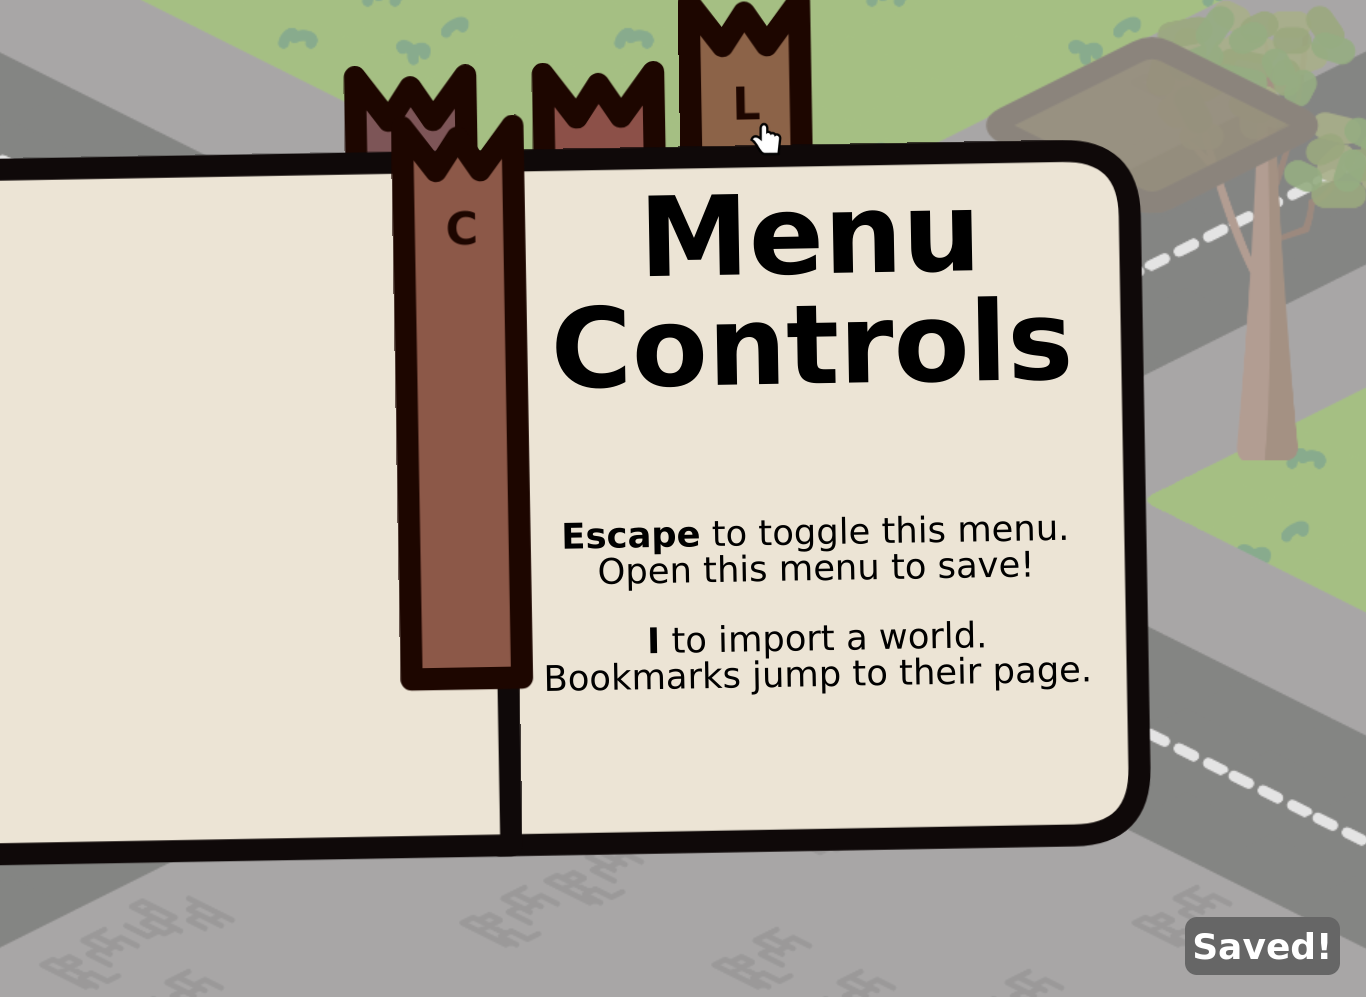
\includegraphics[width=0.8\textwidth]{docs/imgs/UI1.png}};
    \begin{scope}[x={(image.south east)}, y={(image.north west)}]
        \draw[gray, ultra thick] (0.56, 0.86) circle (0.05);
        \node[fill=white, rounded corners] at (0.6, 0.8) {Clickable bookmarks with hover};
        \draw[latex-, ultra thick, black] (0.3, 0.4) -- (0.1, 0.25)
            node[below, color=black] {Current page's bookmark};
        \node[fill=white, rounded corners] at (0.7, 0.29) {Clear information on each page of book};
    \end{scope}
\end{tikzpicture}\end{center}\end{figure}
\begin{figure}[H]\begin{center}\begin{tikzpicture}
  \node[anchor=south west, inner sep=0] (image) at (0,0) {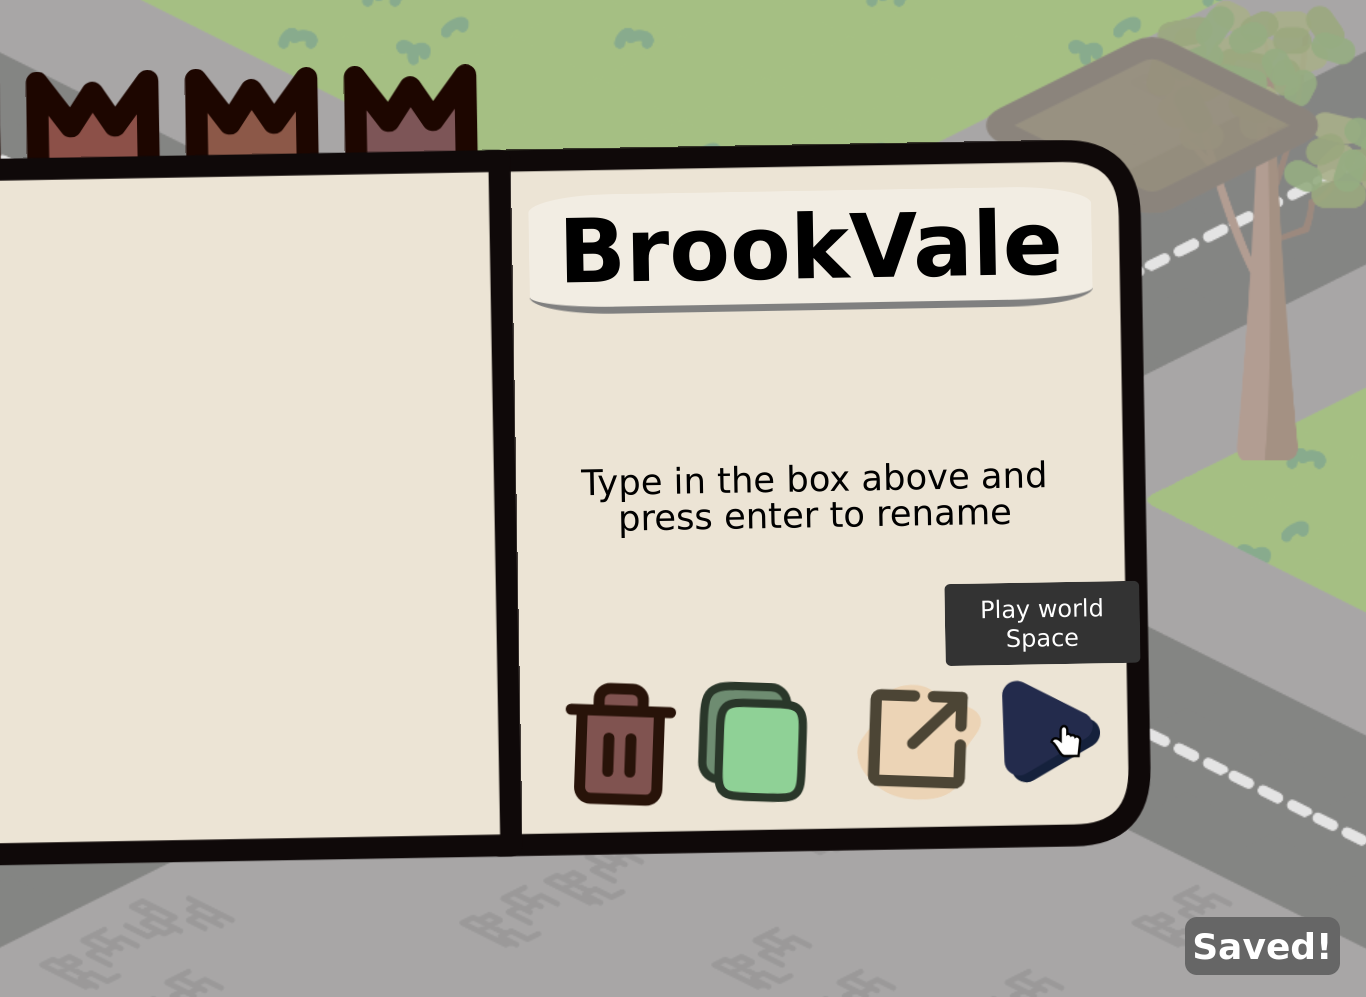
\includegraphics[width=0.8\textwidth]{docs/imgs/UI2.png}};
    \begin{scope}[x={(image.south east)}, y={(image.north west)}]
        \draw[gray, ultra thick] (0.78, 0.25) circle (0.05);
        \node[fill=white, rounded corners] at (0.78, 0.2) {Easy obvious buttons with hover labels};
        \draw[latex-, ultra thick, black] (0.45, 0.5) -- (0.3, 0.4)
            node[below, color=gray] {Clear user instruction when not obvious};
    \end{scope}
\end{tikzpicture}\end{center}\end{figure}
\begin{figure}[H]\begin{center}\begin{tikzpicture}
  \node[anchor=south west, inner sep=0] (image) at (0,0) {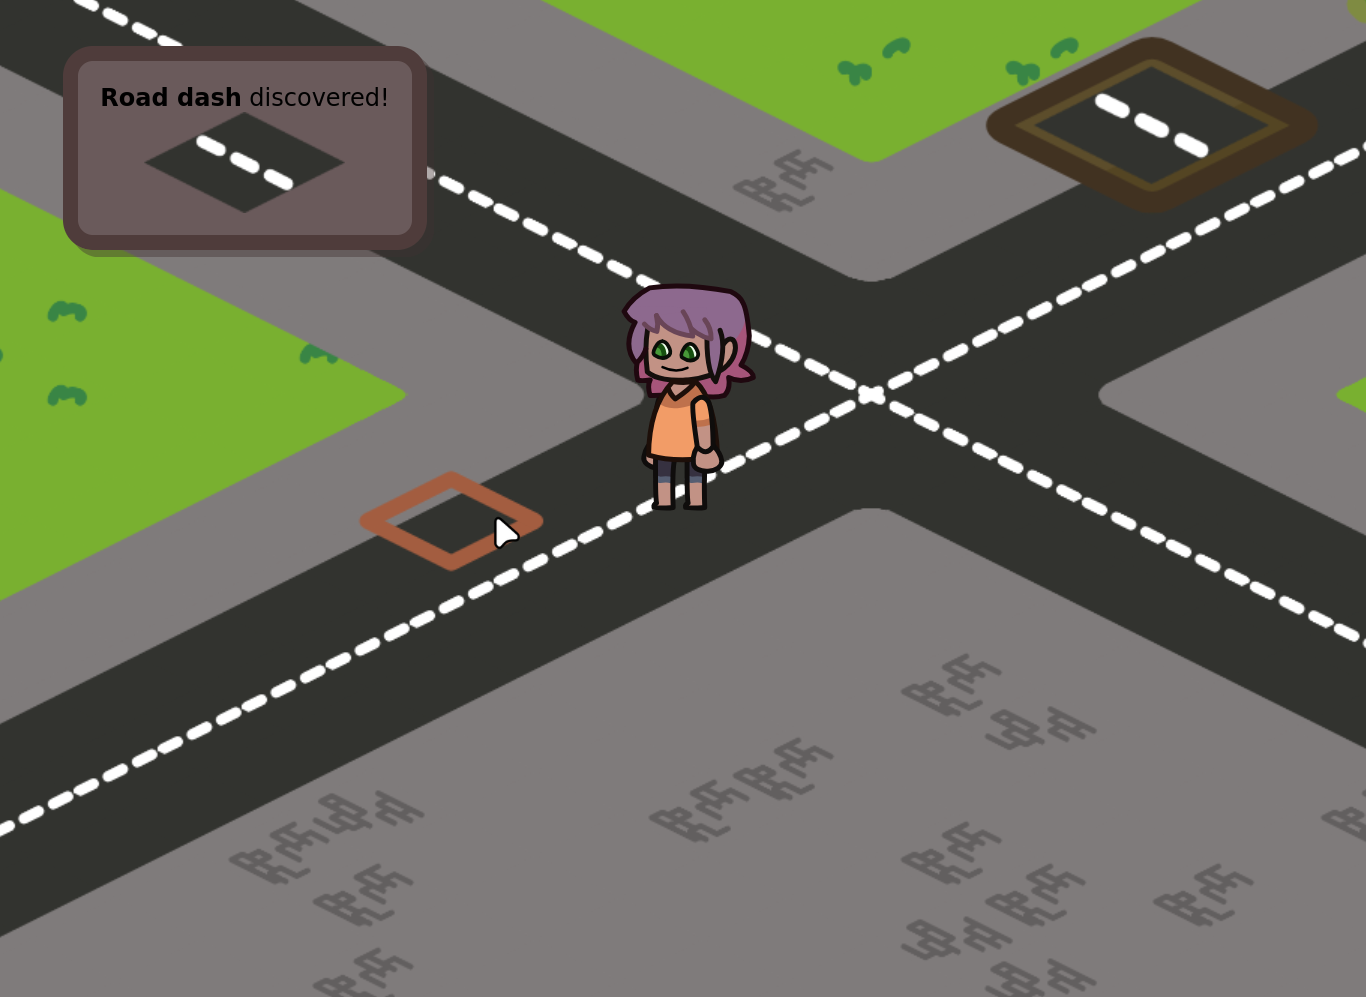
\includegraphics[width=0.8\textwidth]{docs/imgs/UI3.png}};
    \begin{scope}[x={(image.south east)}, y={(image.north west)}]
        \draw[gray, ultra thick] (0.37, 0.47) circle (0.05);
        \node[fill=white, rounded corners] at (0.37, 0.42) {Current tile hover so users know};
        \node[fill=white, rounded corners] at (0.37, 0.38) {what they are doing};
        \node[fill=white, rounded corners] at (0.24, 0.75) {Clear prompts telling the user what happened};
        \node[fill=white, rounded corners] at (0.9, 0.8) {Obvious current tile selection};
    \end{scope}
\end{tikzpicture}\end{center}\end{figure}
\begin{figure}[H]\begin{center}\begin{tikzpicture}
  \node[anchor=south west, inner sep=0] (image) at (0,0) {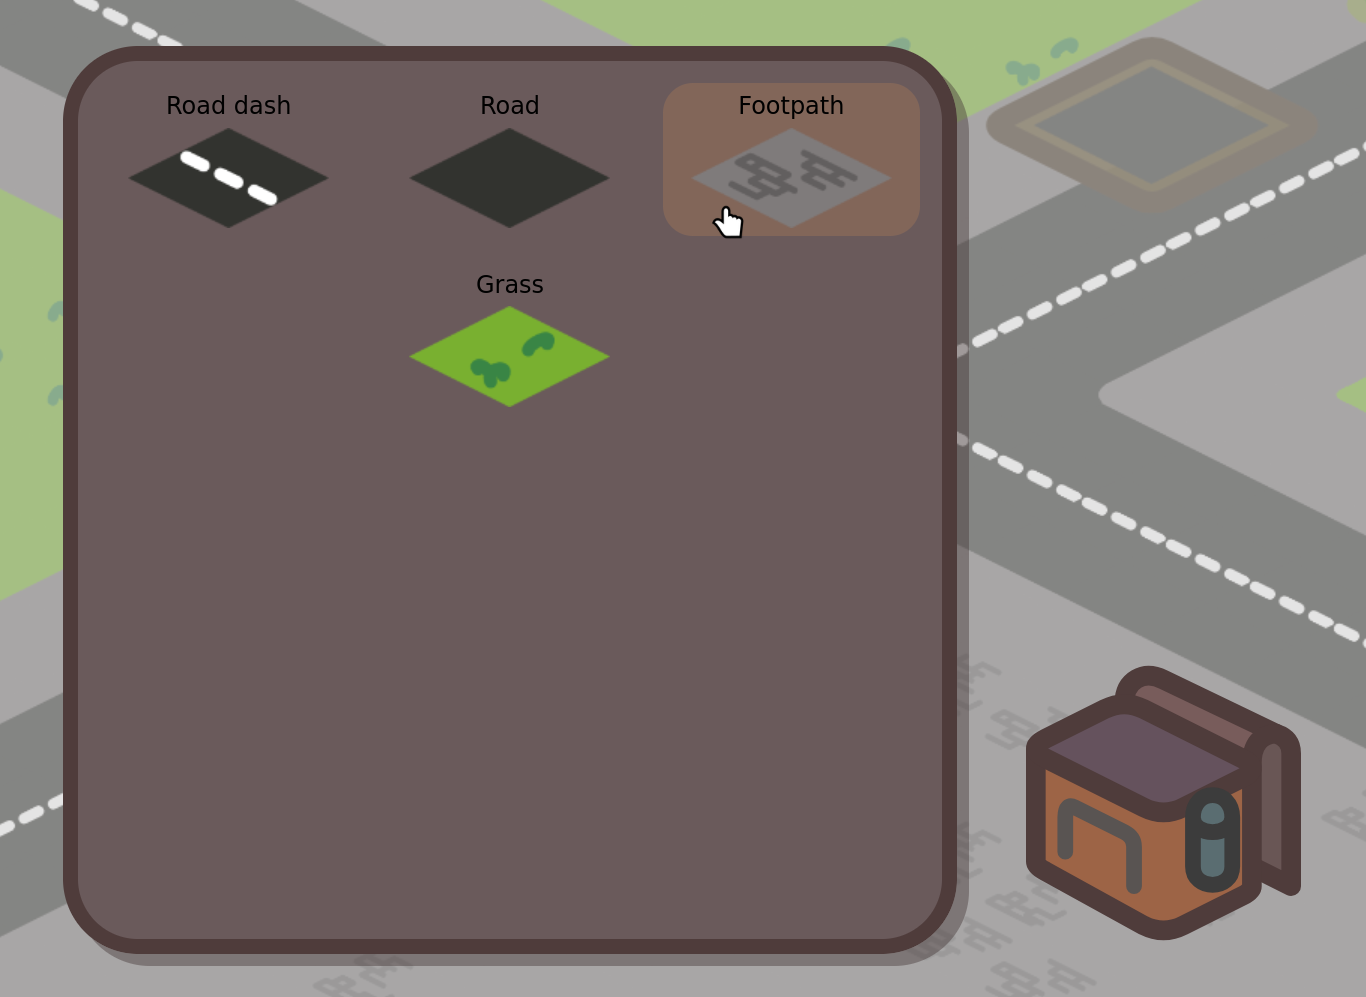
\includegraphics[width=0.8\textwidth]{docs/imgs/UI4.png}};
    \begin{scope}[x={(image.south east)}, y={(image.north west)}]
        \draw[black, ultra thick] (0.53, 0.77) circle (0.05);
        \node[fill=white, rounded corners] at (0.53, 0.72) {Hover effects};
    \end{scope}
\end{tikzpicture}\end{center}\end{figure}

\subsection{Version Control Summary}
% Summarise commits, iterations, or sprints if version control was used.
First, the basic tile drawing was implemented.
A loading screen was then added.
Then implemented movement and finished the basic rendering.
Then basic terrain generation was implemented.
Afterwards there was some optimisation and bugfixing.
Improved the generation even more.
Then implemented the player, found out the drawing was slightly off and fixed it.
Added collision between the player and some blocks.
Then implemented multilayer rendering with a tree.
Then some improvements and speed-ups.
Then implemented a block select highlight and hotbar.
Also improved controls too.
Made picking up blocks better and added placing blocks.
Slightly improved some things.
Then added a journal as an intro to the game with bookmarks and world loading capabilities.
Then added saving and loading worlds.
Stored placed tiles in world info.
Various minor improvements and bugfixes.
Added rename and delete world capabilities.
More various minor improvements.
Added another page for controls, improving backend page usage.
Various minor improvements.
Spent a while implementing a rule-based tile generation.
Various minor Improvements and fixes.
Added export and import with encryption.
Various improvements and extremely minor features.
Made menuing easier.
Many minor improvements and fixes.
Added a find block system instead of cycling with a backpack.
Major backend fixes to the journal.
Minor improvements and fixes, and added compilation to make loading faster.


\section{Testing and Evaluation}

\subsection{Testing Methods Used}
% Describe testing approaches, such as:
    % Unit testing, Integration testing, User testing
% Explain how testing results were used to improve performance, efficiency, or reliability.
Testing was done through unit, system and user tests.
To ensure different parts were working, the codebase was stripped of features that got in the way of the test (for example, occasionally the generation algorithm was stripped down to alternating tiles for clearer visibility of tile boundaries) and the unit tests were conducted through repeatedly doing the same action and verifying it matches with the expected outcomes. These unit tests both made features more reliable and more efficient, as bugs were ironed out and inefficiencies were spotted and dealt with.

There were no integration tests done as the different parts ran separately, without needing to collaborate. Because some modules rely on functions from others, the parts with no dependencies were tested first before progressively testing the other units separately to ensure everything works.

There was system and user testing to ensure the system worked all together as expected, as when there were issues, the parts where the problem occurred were singled out and subject to more extensive unit testing. This allowed for even more performance and reliability increases as more issues were discovered due to seeing everything work together. User testing additionally improved parts of the UX design that were inefficient or difficult to understand.

\subsection{Test Cases and Results}
% Table containing Test ID, Description, Expected Result, Actual Result, Pass/Fail
\begin{brtbl}{|X|X|X|X|X|}{3}{ Test ID & Description & Expected result & Actual result & Pass/fail }
  T01 & Test movement speed of the player &
  The movement should be the same speed no matter what direction is being pressed, including diagonals &
  The player does move at a consistent speed & Pass
\\ \hline
  T02 & Test collision &
  When walking diagonally into a tile with collision the player should slide off at the same speed as movement, and when walking perpendicular into the block the player should be stopped. &
  This does happen & Pass
\\ \hline
  T03 & Test 
\end{brtbl}

\subsection{Evaluation Against Requirements}
% Evaluate how effectively the solution meets the identified functional and non-functional requirements. Consider your ongoing quality assurance processes.
% Evaluate your project in terms of how effectively you addressed compliance and legislative requirements (consider privacy, use of data, etc).
The game effectively meets almost all functional and non-functional requirements satisfactorily. The game's visuals provide a relaxing atmosphere and users are able to make new worlds, export, import and load worlds, among even more world management features, in a clean and efficient manner. Worlds are exported with a password for security when sharing online, and changes made to worlds can be saved. Users are also able to move and add/remove tiles in the world and are guided on how to do so by a controls screen. This means all functional requirements are achieved satisfactorily.

The non-functional requirements are almost fully satisfied. The game stores data in local storage, which other apps cannot access - making it secure from other websites and users (as it is in the user's config which other users on the same computer cannot access without permission). The game was designed to conform to any sized screen (including mobile sizes) and work on any modern browser, and does not detriment from user experience when running into unhandled errors. Bugs and crashes additionally do not occur during normal gameplay. With loading, while chunks are loaded quickly and efficiently offscreen and worlds load within a second, the game does not start within 2 seconds unless it has already loaded before and assets have been cached. But this is ok, as it does not take a long time to load the first time and subsequent loads are still within 2 seconds - meaning overall, the solution meets almost all the identified requirements satisfactorily.

\subsection{Improvements and Future Development}
% Outline your project’s limitations.
% Explain realistic future enhancements.
The project was limited as procedural generation requires a lot of variety to look good, and while I have some it can get a bit boring over time. Easy future improvements would be better procedural generative algorithms and more tiles and decorations. This is where I would draw more tiles and decorations and improve the generation algorithm to generate more interestingly shaped or varied terrain. This would add a significant more amount of variety to make the game more interesting.

\subsection{Evaluation of Social, Ethical and Communication Issues}
% Evaluate your project in terms of


\section{Feedback, Security and Reflection}

\subsection{Summary of Peer Feedback}
% Summarise feedback received and explain how it influenced development.
    % You could collect a ‘PMI’ (Plus, Minus, Implication) table from at least three different people after testing, or record and summarise an interview with at least three three people who test the software.
% Evaluate your use of feedback to improve your project:
    % Consider your individual workflow and how well you responded to peer / stakeholder feedback
    % Consider how well you involved, empowered or negotiated with a peer/client throughout the process.

\subsubsection{Peer feedback throughout development}
\begin{itemize}
  \item One user was trying to click various UI elements expecting them to do something when they did not (for example the current selected block in the top right), so I added in that functionality to make the app more flexible for users who do not find the controls I set convenient.
  \item Throughout development I had a 'cycle' system for tiles, where clicking on a block cycled through all the things that were on that tile. This was not explained well (there wasn't much space to explain it in the intro screen anyway) and was confusing even when I explained it in person. I also planned on implementing a backpack system anyway, so I removed this in favour of a 'block discovery' system. This made selecting blocks much more intuative.
  \item There was much confusion around the traffic cone tile as I drew it slightly odd, and many people thought it looked like a pizza slice. This was remedied later in development.
\end{itemize}

\subsubsection{Peer feedback of final product}
\begin{brtbl}{|X|X|}{2}{ Positives & Negatives, Implications \& Future improvements }
  \multicolumn{2}{|c|}{\textbf{Miles}} \\ \hline
  \begin{itemize}[topsep=0pt, label=+]
    \item Intuative Keybinds
    \item Great Asset Design
    \item Good Movement Controls
  \end{itemize} &
  \begin{itemize}[topsep=0pt, label=-]
    \item No Animations for Legs
    \item Map Feels Repedative between Load files
    \begin{itemize}[topsep=0pt, label=$\rightarrow$]
      \item Made the range of items feel less special in a way
    \end{itemize}
  \end{itemize}
  \begin{itemize}[topsep=0pt]
    \item Could add houses
  \end{itemize} \\ \hline\hline

  \multicolumn{2}{|c|}{\textbf{Oliver}} \\ \hline
  \begin{itemize}[topsep=0pt, label=+]
    \item Everything works great together
    \item Couldn't find any bugs
    \item Cool tile interactions (for example the road lines and water)
    \item Very enjoyable, nice and relaxing
  \end{itemize} &
  \begin{itemize}[topsep=0pt, label=-]
    \item Not enough area types, but didn't detract from the overall feel much.
  \end{itemize}
\end{brtbl}

\subsection{Secure Software Design and Data Handling}
% Evaluate the approach undertaken to safely and securely collect, use, and store data.
    % Your evaluation should address:
        % Secure coding practices applied during development
        % Input validation and error handling
        % Data storage and protection methods
        % The impact of secure software design on user trust, data integrity, and system reliability
During development, the code was developed securely so no other websites could change the data.
All inputs and the URL itself does not get executed, meaning attackers cannot use XSS.
Additionally, save data is stored in the localstorage, meaning no other websites can access the data.
Encryption was also utilised on exports so users can have an extra layer of security when sharing.

All these security aspects ensure the data is never accessible to attackers from within the browser, which increases system reliability and integrity as data breaches and hacks are much less likely, which in turn improves user trust.

\subsection{Personal Reflection}
% Reflect on what you learned during the project, including
    % Software engineering skills developed
    % Challenges encountered and how they were overcome
During the project I improved my skills in web dev and maths. I hadn't done much web dev before, so I was constantly researching how to do simple things in JS or HTML or CSS and from that I learnt many common features of the languages and now can make future projects faster.

Most struggles I had during the project were to do with maths, where I would work out how something should be done but after implementation it doesn't work. These were overcome through much trial and error and more thinking over the problems until eventually I found something that worked.


\end{document}
